\chapter{Algoritmi randomizzati e RandQS}
\label{cha:randqs}

\scan{51}Con questa lezione si apre la seconda parte del corso, dedicata agli
\emph{algoritmi randomizzati}. Riferimenti bibliografici:
\begin{itemize}
  \item \emph{Randomized Algorithms}, di Motwani e Raghavan --- interessante,
        con molti conti da fare;
  \item \emph{An introduction to randomized algorithms}, di Richard Karp.
\end{itemize}

\section{Che cos'è un algoritmo randomizzato}
\label{sec:def-randomizzato}

\begin{definizione}[Algoritmo randomizzato]
\label{def:algoritmo-randomizzato}
Un \emph{algoritmo randomizzato} è un algoritmo che riceve, oltre al proprio
input, un \emph{flusso} (\emph{stream}) di \emph{bit casuali} che utilizza per
compiere \emph{scelte casuali}.
\end{definizione}

\begin{osservazione}
Il flusso non deve essere casuale in senso stretto: basta che sia una sequenza
che l'utente non è in grado di distinguere da una sequenza random.
\end{osservazione}

\begin{figure}[H]
  \centering
  % rand-schema-bit -- pag. 51
% Un algoritmo randomizzato riceve, accanto al proprio input, un flusso di bit
% casuali; poiche' le scelte compiute dipendono da quei bit, la complessita'
% dell'esecuzione (e in generale anche il risultato) e' una variabile aleatoria.
\begin{tikzpicture}[
    x=1cm, y=1cm, >=Latex,
    filo/.style={draw=black!80,line width=0.7pt},
    et/.style={font=\small}
  ]

  % ---- la scatola dell'algoritmo -------------------------------------------
  \node[draw=black!80,line width=1pt,minimum width=2.2cm,minimum height=1.5cm,
        inner sep=2pt,font=\small] (alg) at (0,0) {algoritmo};

  % ---- il flusso di bit casuali --------------------------------------------
  \node[et,align=center,anchor=south] (bit) at (-3.55,1.30)
        {\texttt{010110}\\[-2pt] \emph{random}};
  \draw[filo,->] (bit.south) to[out=-90,in=180] (-1.15,0.35);

  % ---- l'input ordinario ---------------------------------------------------
  \node[et,anchor=east] (in) at (-3.00,-0.40) {input};
  \draw[filo,->] (in.east) -- (-1.15,-0.40);

  % ---- l'uscita: la complessita' e' una variabile aleatoria -----------------
  \draw[filo,->] (1.15,0.20) to[out=0,in=90] (2.90,-1.40);
  \node[et,anchor=west] at (3.05,-0.60) {complessit\`a};

\end{tikzpicture}

  \caption{Un algoritmo randomizzato riceve in ingresso, accanto all'input, un
  flusso di bit casuali; di conseguenza anche la complessità dell'esecuzione
  diventa una variabile aleatoria.}
  \label{fig:rand-schema-bit}
\end{figure}

Poiché le scelte compiute dipendono dai bit casuali, sia il risultato prodotto
sia la complessità dell'esecuzione diventano variabili aleatorie. Fissando
l'una o l'altra si ottengono le due famiglie classiche:
\begin{itemize}
  \item \MonteCarlo: risultato potenzialmente sbagliato, complessità fissa;
  \item \LasVegas: complessità variabile, risultato sempre corretto.
\end{itemize}

Il primo esempio che incontreremo, \RandQS, appartiene alla seconda famiglia:
l'output è sempre l'insieme ordinato, mentre il numero di operazioni eseguite
dipende dalle scelte casuali ed è quindi una variabile aleatoria. Il taglio
minimo, di cui ci occuperemo subito dopo, è invece l'esempio prototipico della
prima.

\section{Randomized QuickSort}
\label{sec:randqs}

\scan{52}L'idea di \RandQS è quella di QuickSort, con un'unica differenza: il pivot non
viene scelto in modo deterministico (il primo elemento, l'ultimo, la mediana di
tre, \dots), ma viene \emph{estratto uniformemente a caso} dall'insieme da
ordinare.

\begin{algorithm}[H]
\caption{\RandQS}
\begin{algorithmic}[1]
\Require un insieme di numeri $S$ (elementi distinti)
\Ensure gli elementi di $S$ in ordine crescente
\State scegli un elemento $x \in S$ \textbf{uniformemente a caso};
\State $\textsc{Partition}(S,x)$: genera $S_1=\set{y\in S \mid y<x}$ e
       $S_2=\set{y\in S \mid y>x}$;
\State ordina ricorsivamente con \RandQS{}($S_1$) e \RandQS{}($S_2$); restituisci
       $S_1$ ordinato, seguito da $x$, seguito da $S_2$ ordinato.
\end{algorithmic}
\end{algorithm}

\begin{osservazione}
QuickSort ha complessità $\Oh(n\log n)$ nel caso medio \emph{se la distribuzione
degli input è uniforme}: si tratta di un'ipotesi (forte) sui possibili input.
\RandQS, invece, \textbf{non} fa alcuna ipotesi sulla distribuzione dell'input:
la casualità non sta più nei dati, ma nell'algoritmo.
\end{osservazione}

\subsection{Il caso ideale}
\label{sec:randqs-caso-ideale}

Nel caso ideale il pivot cade «in mezzo» e la partizione produce due
sottoproblemi di $n/2$ elementi ciascuno.

\begin{figure}[H]
  \centering
  % randqs-partizione -- pag. 52
% Caso ideale: il pivot estratto uniformemente a caso spezza S in due
% sottoinsiemi di n/2 elementi; le due frecce sono le chiamate ricorsive
% RandQS(S_1) e RandQS(S_2). E' la figura che giustifica T(n)=O(n)+2T(n/2).
\begin{tikzpicture}[
    x=1cm, y=1cm, >=Latex,
    filo/.style={draw=black!80,line width=0.8pt},
    et/.style={font=\footnotesize}
  ]

  % ---- la cella del pivot ---------------------------------------------------
  \draw[filo,line width=1pt] (-0.28,1.92) rectangle (0.28,2.48);
  \node[et,anchor=south] at (0,2.58) {pivot};

  % ---- le due chiamate ricorsive -------------------------------------------
  \draw[filo,->] (-0.28,1.92) to[out=-120,in=60]  (-2.10,0.55);
  \draw[filo,->] ( 0.28,1.92) to[out=-60, in=120] ( 2.10,0.55);

  % ---- i due sottoinsiemi, di n/2 elementi ciascuno -------------------------
  \foreach \c in {-2.10, 2.10} {
    \draw[filo] (\c-1.5,-0.22) rectangle (\c+1.5,0.22);
    \draw[filo] (\c-1.5,-0.36) -- (\c-1.5,0.36);
    \draw[filo] (\c+1.5,-0.36) -- (\c+1.5,0.36);
    \node at (\c,0) {$n/2$};
  }

\end{tikzpicture}

  \caption{Partizione ideale: il pivot spezza l'insieme in due metà di $n/2$
  elementi.}
  \label{fig:randqs-partizione}
\end{figure}

In questo caso l'albero delle chiamate ricorsive è bilanciato: ha altezza
$h=\log_2 n$ e ad ogni livello il costo complessivo delle partizioni è
$\Oh(n)$, perché i sottoproblemi di uno stesso livello ripartiscono fra loro gli
$n$ elementi di partenza.

\begin{figure}[H]
  \centering
  % randqs-albero-chiamate -- pag. 52
% Albero delle chiamate ricorsive nel caso bilanciato: e' un albero binario
% completo di altezza h = log_2 n; su ogni livello i sottoproblemi si
% ripartiscono gli n elementi, quindi il costo per livello e' O(n).
\begin{tikzpicture}[
    x=1cm, y=1cm, >=Latex,
    filo/.style={draw=black!80,line width=0.7pt},
    nodo/.style={circle,draw=black!80,fill=white,line width=0.7pt,
                 inner sep=0pt,minimum size=4.5pt},
    radice/.style={circle,draw=black!80,fill=black!80,inner sep=0pt,
                   minimum size=5.5pt},
    onda/.style={filo,->,decorate,
                 decoration={snake,amplitude=0.5mm,segment length=3mm,
                             post length=2mm,pre length=1mm}}
  ]

  % ---- i nodi ---------------------------------------------------------------
  \node[radice] (r)  at ( 0.00,2.40) {};
  \node[nodo]   (a)  at (-1.15,1.20) {};
  \node[nodo]   (b)  at ( 1.15,1.20) {};
  \node[nodo]   (a1) at (-1.75,0.00) {};
  \node[nodo]   (a2) at (-0.55,0.00) {};
  \node[nodo]   (b1) at ( 0.55,0.00) {};
  \node[nodo]   (b2) at ( 1.75,0.00) {};

  % ---- gli archi ------------------------------------------------------------
  \draw[filo] (r) -- (a);   \draw[filo] (r) -- (b);
  \draw[filo] (a) -- (a1);  \draw[filo] (a) -- (a2);
  \draw[filo] (b) -- (b1);  \draw[filo] (b) -- (b2);

  % ---- l'altezza dell'albero ------------------------------------------------
  \draw[filo,decorate,decoration={brace,amplitude=6pt}]
       (-2.60,-0.18) -- (-2.60,2.58);
  \node[anchor=east] at (-2.85,1.20) {$h$};

  % ---- il costo di ciascun livello ------------------------------------------
  \draw[onda] (0.25,2.40) -- (2.80,2.40);
  \draw[onda] (1.40,1.20) -- (2.80,1.20);
  \draw[onda] (1.95,0.00) -- (2.80,0.00);
  \node[anchor=west] at (2.95,2.40) {$\Oh(n)$};
  \node[anchor=west] at (2.95,1.20) {$\Oh(n)$};
  \node[anchor=west] at (2.95,0.00) {$\Oh(n)$};

\end{tikzpicture}

  \caption{Albero delle chiamate ricorsive nel caso bilanciato: $h=\log_2 n$
  livelli, ciascuno di costo complessivo $\Oh(n)$.}
  \label{fig:randqs-albero-chiamate}
\end{figure}

\[
  T(n) \;=\; \Oh(n) \;+\; 2\,T\!\left(\frac{n}{2}\right)
  \qquad\Longrightarrow\qquad
  T(n) \in \Oh(n\log n).
\]

Nulla garantisce però che il pivot estratto a caso spezzi davvero l'insieme in
due metà: la ricorrenza qui sopra vale solo nel caso bilanciato, mentre in
generale una partizione in $p$ e $q$ elementi dà $T(n)=T(p)+T(q)+\Th(n)$, che
nel caso pessimo (pivot sempre estremo) degenera in $\Th(n^2)$. Quello che
possiamo controllare non è dunque il costo di una singola esecuzione, ma il suo
\emph{valore atteso}.

\section{Analisi di \texorpdfstring{\RandQS}{RandQS} nel caso medio}
\label{sec:randqs-analisi}

Qui «caso medio» va inteso come \emph{valore atteso} di una variabile aleatoria
--- quella che rappresenta la complessità --- dove la media è presa sulle scelte
casuali dell'algoritmo, a input fissato, e non sugli input. Non si tratta quindi
dell'analisi di QuickSort nel caso medio: non c'è alcuna ipotesi sulla
distribuzione degli input.

Il costo di \RandQS è dominato dal numero di \emph{confronti} eseguiti dalle
chiamate a \textsc{Partition}: è quello che conteremo.

\begin{teorema}[Numero atteso di confronti di \RandQS]
\label{thm:randqs-confronti}
Il numero atteso di confronti eseguiti da \RandQS su un insieme di $n$ elementi
distinti è al più $2\,n\,H_n$, dove $H_n=\sum_{k=1}^{n}1/k$ è l'$n$-esimo numero
armonico. Poiché $H_n \in \Th(\log n)$, il numero atteso di confronti è
$\Oh(n\log n)$.
\end{teorema}

Indichiamo con $x_i$ l'elemento di rango $i$, cioè l'$i$-esimo elemento di $S$
nell'ordine crescente, e introduciamo per ogni coppia $1\le i<j\le n$ la
variabile aleatoria \emph{indicatrice}
\[
  X_{ij} \;=\;
  \begin{cases}
    1 & \text{se } x_i \text{ \emph{è confrontato} con } x_j,\\[2pt]
    0 & \text{altrimenti,}
  \end{cases}
  \qquad\text{ovvero}\qquad
  X_{ij} = \indic{x_i \text{ è confrontato con } x_j}.
\]

Il numero totale di confronti è allora $\sum_{i=1}^{n}\sum_{j>i} X_{ij}$, e la
quantità da stimare è
\[
  \E\!\left[\; \sum_{i=1}^{n}\sum_{j>i} X_{ij} \;\right].
\]

\subsection{Linearità del valore atteso}
\label{sec:linearita}

\scan{53}Per linearità del valore atteso --- che non richiede alcuna ipotesi di
indipendenza fra le $X_{ij}$ --- vale
\[
  \E\!\left[\;\sum_{i=1}^{n}\sum_{j>i} X_{ij}\right]
  \;=\;
  \sum_{i=1}^{n}\sum_{j>i} \E\!\left[X_{ij}\right].
\]

Poiché $X_{ij}$ è una variabile indicatrice, posto
$p_{ij} = \Pr\!\left[X_{ij}=1\right]$ si ha
\[
  \E\!\left[X_{ij}\right] \;=\; p_{ij}\cdot 1 \;+\; (1-p_{ij})\cdot 0 \;=\; p_{ij},
\]
dove $p_{ij}$ è dunque la probabilità che $x_i$ e $x_j$ vengano confrontati.

\subsection{Calcolo di \texorpdfstring{$p_{ij}$}{p\_ij}}
\label{sec:pij}

Occorre calcolare la probabilità che $x_i$ e $x_j$ siano coinvolti in un
confronto.

\begin{figure}[H]
  \centering
  % randqs-separazione -- pag. 53
% La retta tratteggiata e' la sequenza ordinata x_1 < x_2 < ... < x_n. Se il
% pivot estratto cade strettamente fra x_i e x_j, allora x_i finisce in S_1 e
% x_j in S_2: i due non verranno mai piu' confrontati (evento complementare a
% quello che definisce X_{ij}=1).
\begin{tikzpicture}[
    x=1cm, y=1cm, >=Latex,
    filo/.style={draw=black!80,line width=0.7pt},
    zig/.style={filo,->,decorate,
                decoration={snake,amplitude=0.9mm,segment length=3.6mm,
                            post length=2.5mm}}
  ]

  % ---- la sequenza ordinata degli elementi ---------------------------------
  \draw[filo,dash pattern=on 4pt off 4pt] (-5.4,0) -- (5.4,0);

  % ---- i due elementi x_i e x_j (il tratteggio si interrompe attorno) -------
  \node[fill=white,inner sep=2pt] at (-2.2,0) {$x_i$};
  \node[fill=white,inner sep=2pt] at ( 2.2,0) {$x_j$};

  % ---- il pivot estratto, strettamente compreso fra i due -------------------
  \fill[white] (0,0) circle (5pt);
  \draw[filo] (0,0) circle (2pt);

  % ---- la scelta casuale del pivot ------------------------------------------
  \draw[zig] (0,-1.75) -- (0,-0.10);
  \node[font=\footnotesize,anchor=north] at (0,-1.90) {pivot scelto};

\end{tikzpicture}

  \caption{Se il pivot estratto cade strettamente fra $x_i$ e $x_j$, i due
  elementi finiscono in sottoinsiemi diversi e non verranno mai confrontati.}
  \label{fig:randqs-separazione}
\end{figure}

\begin{osservazione}
$x_i$ e $x_j$ \emph{non} vengono confrontati se il pivot scelto è in
$\set{x_{i+1},\dots,x_{j-1}}$: un pivot interno all'intervallo separa i due
elementi, mandandone uno in $S_1$ e l'altro in $S_2$, e da quel momento in poi
non potranno più essere confrontati.
\end{osservazione}

Ogni elemento $d \in \set{x_i,\dots,x_j}$ ha la stessa probabilità di essere
scelto come pivot; quindi la probabilità di scegliere $x_i$ oppure $x_j$ ---
cioè $p_{ij}$ --- soddisfa
\[
  p_{ij} \;\le\; \frac{2}{\,j-i+1\,}
\]
(è il caso peggiore, quello in cui mi ritrovo con una partizione contenente
esclusivamente $\set{x_i,\dots,x_j}$; generalmente mi ritrovo in partizioni più
grandi, e la probabilità di pescare proprio uno dei due estremi è minore).

\begin{osservazione}
In realtà vale l'uguaglianza $p_{ij} = \dfrac{2}{j-i+1}$. Finché nessuno fra
$x_i, x_{i+1},\dots,x_j$ è stato scelto come pivot, questi $j-i+1$ elementi
stanno tutti nella stessa partizione (un pivot esterno all'intervallo non può
separarli); il primo di essi a diventare pivot è uniformemente distribuito fra i
$j-i+1$ candidati, e $x_i$ e $x_j$ vengono confrontati esattamente quando tale
primo elemento è uno dei due estremi. Per la maggiorazione che segue basta
comunque la disuguaglianza.
\end{osservazione}

Sommando su tutte le coppie, e osservando che per $i$ fissato il denominatore
$j-i+1$ percorre i valori $2,3,\dots,n-i+1$:
\[
  \sum_{i=1}^{n}\sum_{j>i} p_{ij}
  \;\le\; \sum_{i=1}^{n}\sum_{j>i} \frac{2}{\,j-i+1\,}
  \;\le\; 2\sum_{i=1}^{n} \underbrace{\sum_{k=1}^{n}\frac{1}{k}}_{H_n}
  \;=\; 2\sum_{i=1}^{n} H_n
  \;=\; 2\,n\,H_n .
\]

\subsection{Il numero armonico}
\label{sec:numero-armonico}

\[
  H_n \;=\; \sum_{k=1}^{n}\frac1k
  \;=\; 1+\frac12+\frac13+\frac14+\frac15+\frac16+\frac17+\cdots
\]
Raggruppando i termini a blocchi di lunghezza $1,2,4,8,\dots$ --- i blocchi sono
$\lfloor\log_2 n\rfloor+1$ e ogni blocco \emph{completo} ha somma compresa fra
$1/2$ e $1$, mentre l'ultimo può essere parziale --- si ottengono le due stime,
la seconda con i blocchi traslati di un posto:
\begin{align*}
  H_n &\;=\; 1
    + \underbrace{\left(\frac12+\frac13\right)}_{\le\;\frac12+\frac12\;=\;1}
    + \underbrace{\left(\frac14+\frac15+\frac16+\frac17\right)}_{\le\;4\cdot\frac14\;=\;1}
    + \cdots \;\le\; 1+\log_2 n, \\[6pt]
  H_n &\;=\; 1+\frac12
    + \underbrace{\left(\frac13+\frac14\right)}_{\ge\;\frac14+\frac14\;=\;\frac12}
    + \underbrace{\left(\frac15+\frac16+\frac17+\frac18\right)}_{\ge\;4\cdot\frac18\;=\;\frac12}
    + \cdots \;\ge\; \frac12\log_2 n .
\end{align*}

Dunque $H_n \in \Th(\log n)$ e, mettendo insieme i pezzi,
\[
  \E\!\left[\;\sum_{i=1}^{n}\sum_{j>i} X_{ij}\;\right]
  \;=\; \sum_{i=1}^{n}\sum_{j>i} p_{ij}
  \;\le\; 2\,n\,H_n \;\in\; \Th(n\log n),
\]
cioè il numero atteso di confronti di \RandQS è $\Oh(n\log n)$, come annunciato
dal Teorema~\ref{thm:randqs-confronti}.

\begin{osservazione}
Ogni scelta del pivot viene pagata in bit casuali: per estrarre uniformemente un
elemento da un insieme di $n$ elementi servono $\log_2 n$ bit letti dalla
sorgente,
\[
  \text{scelta del pivot}\;\longleftarrow\;
  \underbrace{0\,1\,0\,1\,0\;\cdots}_{\log_2 n\ \text{bit}}
\]
\end{osservazione}

\subsection{Elementi ripetuti}
\label{sec:randqs-ripetuti}

\scan{54}L'analisi svolta finora suppone che gli elementi da ordinare siano \emph{a due a
due distinti}: è l'ipotesi che rende ben definiti i ranghi $x_1<\dots<x_n$ e che
garantisce $S_1\cup\set{x}\cup S_2 = S$.

\begin{figure}[H]
  \centering
  % randqs-pivot-array -- un passo di RandQS: scelta uniforme del pivot nel segmento.
\begin{tikzpicture}[x=1cm,y=1cm,line join=round,line cap=round]
  \footnotesize
  % --- il segmento corrente: rettangolo allungato, prima e ultima cella marcate
  \draw[thick] (0,0) rectangle (8.4,0.55);
  \draw[thick] (0.6,0) -- (0.6,0.55);
  \draw[thick] (7.8,0) -- (7.8,0.55);

  % --- posizione del pivot (~45% del segmento)
  \coordinate (P) at (3.8,0.61);

  % --- scelta casuale: arco dall'inizio del segmento alla cella del pivot
  \draw[thick,-{Stealth[length=2.4mm,width=2mm]}]
    (0.35,0.75) .. controls (1.1,1.85) and (3.0,1.9) .. (P);
  \node[gray,anchor=south] at (2.1,1.62) {scelta uniforme a caso};

  % --- freccia ondulata dal basso che indica la cella del pivot
  \draw[thick,-{Stealth[length=2.2mm,width=1.8mm]}]
    plot[domain=0:1,samples=90,smooth,variable=\t]
      ({3.8-0.30*(1-\t)+0.10*(1-\t)*sin(\t*1080)},{-1.15+1.03*\t});
  \node[anchor=north east] at (3.62,-1.12) {pivot};
\end{tikzpicture}

  \caption{Un passo di \RandQS: il pivot è scelto uniformemente a caso fra gli
  elementi del segmento corrente, che si assumono a due a due distinti.}
  \label{fig:randqs-pivot-array}
\end{figure}

Se l'input contiene ripetizioni basta sostituire la sequenza $a_1,\dots,a_n$ con
la sequenza di coppie
\[
  \tuple{a_1,1},\ \tuple{a_2,2},\ \dots,\ \tuple{a_n,n},
\]
ordinate lessicograficamente: la seconda componente rende le coppie a due a due
distinte e non altera l'ordine relativo dei valori $a_i$. È una soluzione pulita
e semplice per ripulire l'analisi in presenza di copie ripetute.

\section{Che cosa viene dopo}
\label{sec:randqs-seguito}

\scan{54}Il prossimo problema è quello del \emph{taglio minimo} (\mincut): dato un grafo,
individuare un insieme di archi la cui rimozione lo sconnette e che abbia
cardinalità minima.

\begin{figure}[H]
  \centering
  % mincut-anticipazione -- un taglio di G: la spezzata separa i vertici in due parti,
% il taglio e' l'insieme degli archi che la attraversano.
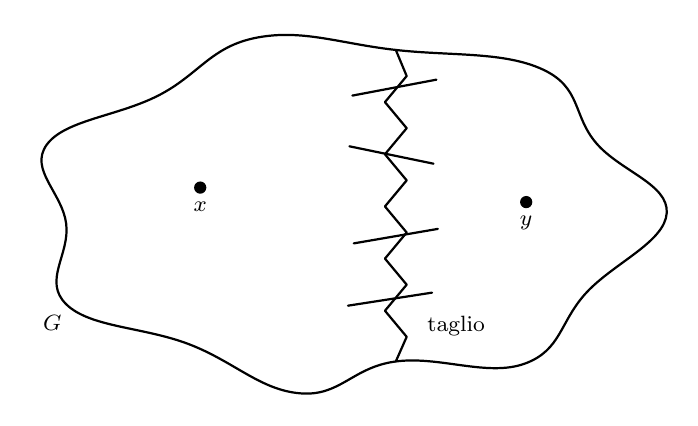
\begin{tikzpicture}[x=1cm,y=1cm,line join=round,line cap=round,scale=0.92]
  \footnotesize
  % --- sagoma del grafo G
  \draw[thick] plot[smooth cycle,tension=0.7] coordinates {
    (4.44,0.00) (3.47,0.96) (2.73,1.98) (0.70,2.25) (-1.22,2.42) (-2.58,1.62)
    (-4.12,0.94) (-3.85,-0.15) (-3.85,-1.26) (-2.16,-1.81) (-0.62,-2.49)
    (0.70,-2.05) (2.48,-2.08) (3.34,-1.09)};
  \node[anchor=north east] at (-3.80,-1.30) {$G$};

  % --- frontiera del taglio: spezzata a zig-zag dal bordo superiore a quello inferiore
  \draw[thick]
    (0.70,2.25) -- (0.85,1.89) -- (0.55,1.53) -- (0.85,1.17) -- (0.55,0.81) --
    (0.85,0.45) -- (0.55,0.09) -- (0.85,-0.27) -- (0.55,-0.63) -- (0.85,-0.99) --
    (0.55,-1.35) -- (0.85,-1.71) -- (0.70,-2.05);

  % --- i quattro archi che attraversano il taglio
  \draw[thick] (0.10,1.62) -- (1.26,1.84);
  \draw[thick] (0.06,0.92) -- (1.22,0.68);
  \draw[thick] (0.12,-0.42) -- (1.28,-0.22);
  \draw[thick] (0.04,-1.28) -- (1.20,-1.10);

  % --- i due vertici separati dal taglio
  \fill (-2.00,0.35) circle (2.4pt) node[anchor=north,yshift=-2pt] {$x$};
  \fill ( 2.50,0.15) circle (2.4pt) node[anchor=north,yshift=-2pt] {$y$};

  % --- etichetta della frontiera
  \node[anchor=west] at (1.02,-1.56) {taglio};
\end{tikzpicture}

  \caption{Un taglio di $G$: la linea spezzata separa i vertici in due parti (da
  un lato $x$, dall'altro $y$); il taglio è l'insieme degli archi che la
  attraversano.}
  \label{fig:mincut-anticipazione}
\end{figure}

\begin{itemize}
  \item esistono algoritmi deterministici, ma estremamente complicati;
  \item c'è un algoritmo randomizzato di prestazioni comparabili e molto
        semplice.
\end{itemize}

Dopo ancora: il \emph{metodo probabilistico}.
